\documentclass[12pt, twoside, letterpaper]{report}
\usepackage[top=2cm,bottom=4cm,left=3cm,right=3cm,asymmetric]{geometry}

\usepackage{fancyhdr}
\pagestyle{fancy}
\fancyfoot[C]{}    
\fancyfoot[LE,RO]{\thepage}        
\fancyhead[RO]{\slshape \rightmark}        
\fancyhead[LE]{\slshape\leftmark}      
\fancyhead[RE,LO]{}  

\usepackage{color}   
\usepackage{hyperref}
\usepackage[utf8x]{inputenc}
\usepackage[italian]{babel}
\usepackage{amsmath, amsthm, amssymb, amsfonts}
\usepackage[breakable]{tcolorbox}
\usepackage{pdfpages}
\usepackage{enumitem}
\usepackage{graphicx}
\graphicspath{ {./img/} }
\newcommand{\img}[3] {
	\begin{figure}[h]
		\caption{#1}
		\centering
		\includegraphics[scale=#2]{#3}\\
	\end{figure}
}

\title{Uso di reti neurali per la classificazione di dati in problemi di medicina legale}
\author{Mario Petruccelli \cr Università degli studi di Milano}
\date{A.A. 2019/2020}

\begin{document}

	\begin{titlepage}
		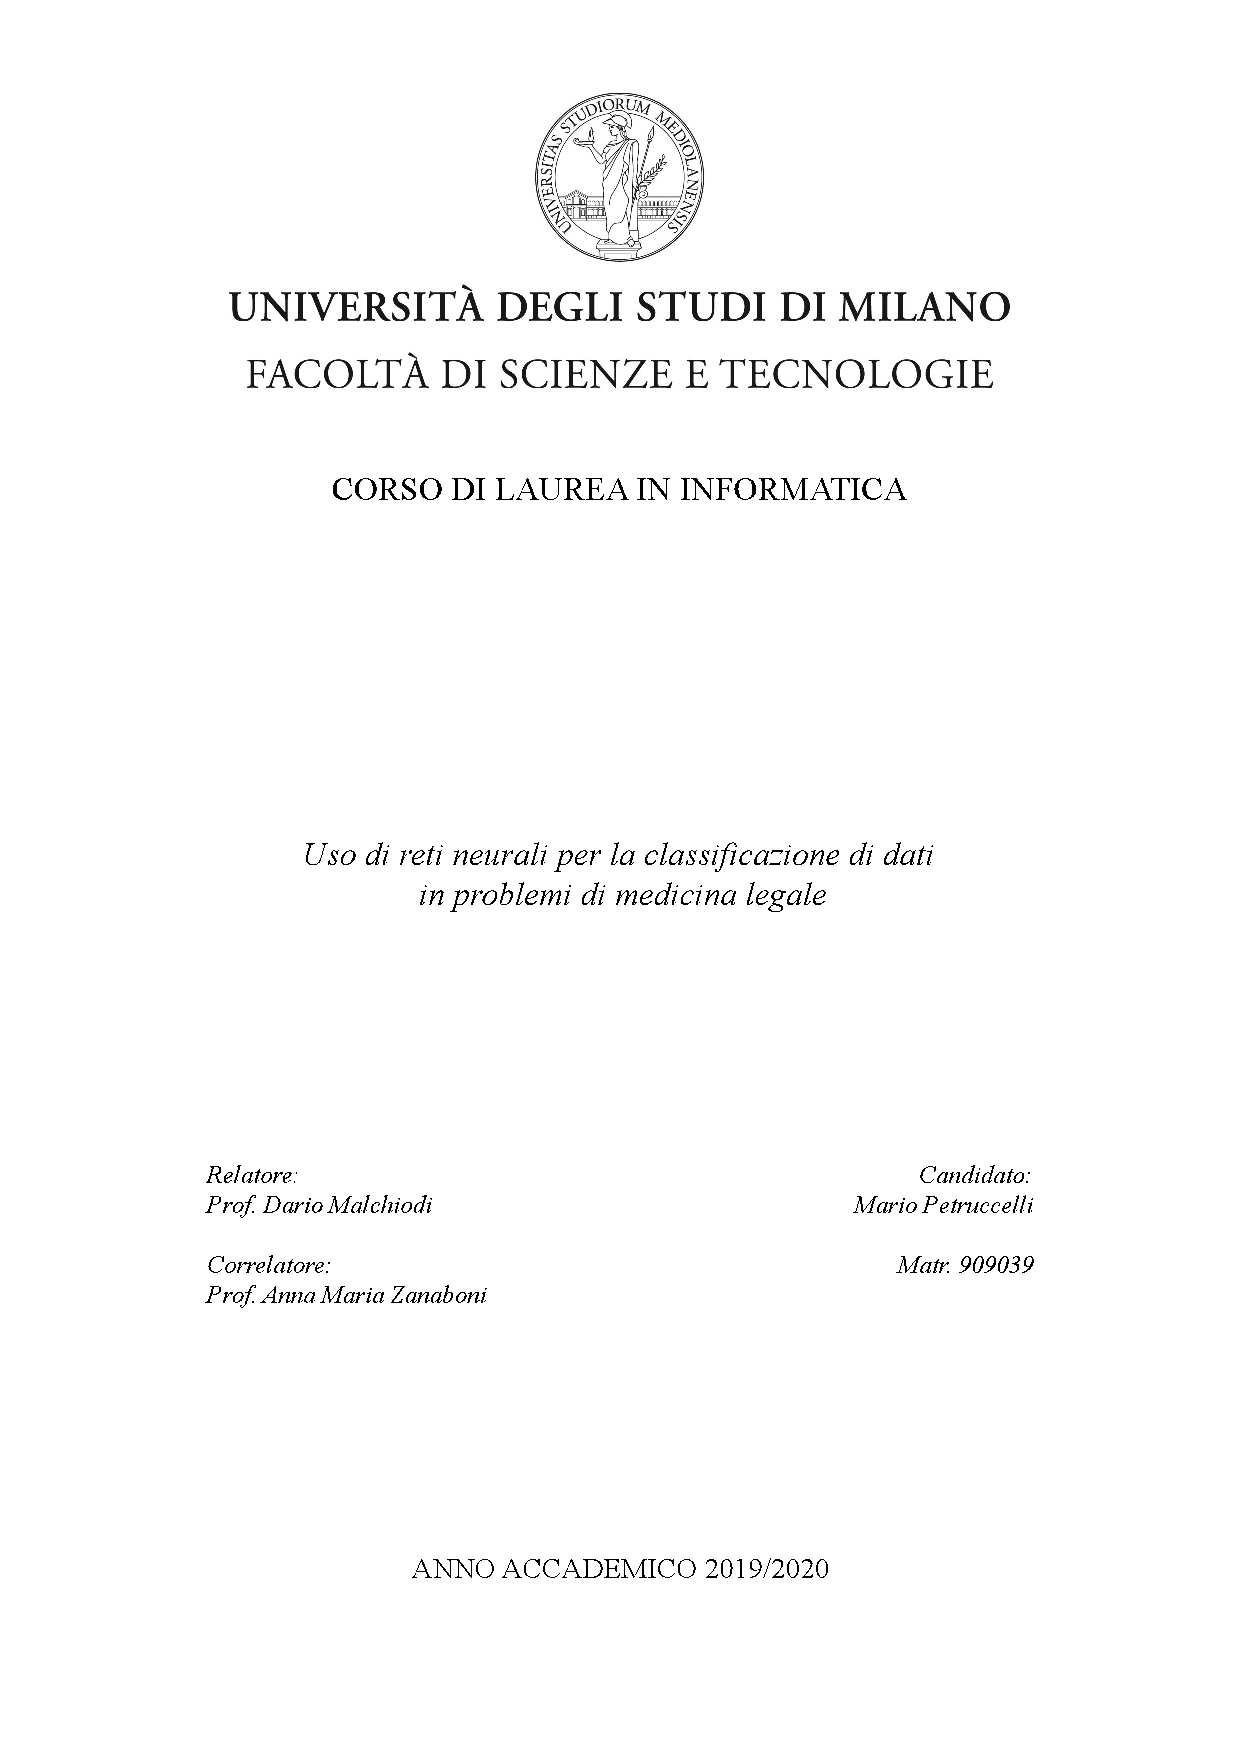
\includepdf{img/FRONTESPIZIO.pdf}
		\newpage
		\tableofcontents
	\end{titlepage}

	\chapter*{Introduzione} \markboth{Introduzione}{}
		Qua ci andrà l'introduzione

		\newpage		
	\chapter{Reti neurali}
		Le \textbf{reti neurali artificiali} sono un campo molto importante del \textit{machine learning}. Consistono in un modello matematico che prende ispirazione dalle reti neurali biologiche, presenti nel cervello animale. In questo capitolo ne vedremo le loro componenti e il loro funzionamento. Ma cos'è il machine learning?

		\section{Paradigma del machine learning}
			Il machine learning è una disciplina scientifica dell'ambito dell'intelligenza artificiale ed è una di quelle in più rapida espansione; negli ultimi decenni è diventato di uso comune in moltissime applicazioni che richiedono l'estrazione di informazioni da dati su larga scala. Lo scopo di tale disciplina è quello di individuare dei pattern significativi nei dati, che difficilmente sarebbero riconoscibili con l'uso tradizionale della programmazione \textit{(e.g. riconoscere la razza di un cane partendo da una foto)}.  
			
			Prendendo come esempio noi umani, molte delle nostre abilità vengono acquisite o raffinate dalla nostra esperienza, e così \textit{impariamo}. Immaginiamo di trovarci in un'isola sperduta e di trovare un albero con frutti mai visti prima. Nonostante questo frutto sia nuovo ai nostri occhi, sapremo riconoscere con molta probabilità se è maturo o acerbo. Lo stesso concetto possiamo provare ad applicarlo alle macchine, ma come possono apprendere? 
			
			\subsection{Tipi di apprendimento} L'apprendimento è un dominio di ampio spettro e di conseguenza, il machine learning è diviso in diversi sottocampi in cui abbiamo più paradigmi di apprendimento. La principale distinzione che possiamo fare è la differenza tra l'apprendimento \textbf{supervisionato} e \textbf{non supervisionato}.
			
				\paragraph{Apprendimento supervisionato} Consideriamo di dover classificare tre specie di fiori leggermente diversi tra loro, appartenenti alla stessa famiglia \textit{(esperimento che riprenderemo più avanti)}. Per imparare a riconoscerli, potremmo ricevere un insieme di dati \textit{(e.g. larghezza dei petali, lunghezza del gambo, ecc...)} appartenenti ai fiori di cui conosciamo già l'etichetta. Dopo questa fase di \textbf{allenamento}, dovremmo essere in grado di trovare un pattern tra i dati per etichettare nuovi fiori, questa volta privi di etichetta e non appartenenti all'insieme dato in precedenza. 
				
					In maniera più astratta, possiamo vedere questo come un processo di \textit{utilizzo dell'esperienza passata per acquisire competenza}. L'apprendimento supervisionato descrive uno scenario in cui l'esperienza, nel nostro caso un insieme di \textbf{training}, contiene delle etichette che non sono presenti nell'insieme di \textbf{test}, a cui dobbiamo applicare l'esperienza acquisita in modo da \textbf{predire} l'informazione mancante.
				
				\paragraph{Apprendimento non supervisionato}  Nell'apprendimento non supervisionato non c'è distinzione tra i dati di training e di test. Vengono processati i dati con lo scopo di tirare fuori una versione compressa, o un "riassunto" di essi. Il raggruppamento dei dati in sottoinsiemi con caratteristiche simili è una delle pratiche più usate in questo campo.\\
				
				Il modello di cui ci occuperemo noi, ovvero le reti neurali artificiali, utilizzano un'apprendimento di tipo supervisionato. Andiamo a vederle più nel dettaglio.
			
		\section{Che cos'è una rete neurale?}
			Come abbiamo già anticipato, le reti neurali artificiali cercano di riprendere quello che sono le loro omonime biologiche. Il cervello animale è un meccanismo in grado di apprendere grazie all'esperienza, ed è per questo che si è cercato di emularlo \textit{(in modo molto semplificato)} come modello di machine learning. Probabilmente saprete già che il cervello è composto da \textbf{neuroni}, ed essi sono connessi tra di loro da delle \textbf{sinapsi} in modo da poter comunicare. Ebbene, anche il nostro modello artificiale riprende questa struttura.
			
			%\img{Rete Neurale}{0.6}{nn.png}
			
		\subsection{Componenti principali di una rete neurale}
			Una rete neurale artificiale può essere vista come un grafo, cioè consiste in un insieme di \textbf{nodi} \textit{(neuroni)} e \textbf{archi orientati pesati} \textit{(sinapsi)}. Più formalmente, una rete neurale è una tripla $(N,V, \omega)$ in cui:
			\begin{itemize}
				\item $N$ è l'insieme dei neuroni.
				\item $V = \{(i,j) | i,j \in N\}$ è l'insieme delle connessioni tra i neuroni $i$ e $j$.
				\item $\omega: V \rightarrow \mathbb{R}$ è la funzione di peso, dove $\omega_{i,j}$ è il peso della connessione tra i neuroni $i$ e $j$.
			\end{itemize}
			Un neurone, per essere definito tale deve essere in grado di elaborare i dati che gli arrivano tramite le sue connessioni. È composto da tre funzioni: funzione di \textbf{propagazione}, funzione di \textbf{attivazione} e funzione di \textbf{output}. 
			
			\img{Struttura di un neurone}{0.4}{neurone.png}
			
			 \paragraph{Funzione di propagazione} Dato un neurone $j$, la sua funzione di propagazione riceve gli output $o_{i_1}, \dots, o_{i_n}$ dei neuroni $i_1, \dots, i_n$ connessi a $j$ e i corrispettivi pesi $\omega_{i,j}$, restituendo un valore detto \textit{network input} net$_j$ che verrà poi processato dalla \textit{funzione di attivazione}. 
			 
			 	Sia $I = \{i_1, i_2, \dots, i_n\}$ l'insieme dei neuroni tale che $\forall z \in \{1, \dots, n\} : \exists w_{i_z,j}$. Allora il network input di $j$ ($net_j$), è calcolato dalla funzione di propagazione $f_{prop}$ come segue: $$net_j = f_{prop}(o_{i_1}, \dots, o_{i_n},w_{i_1,j}, \dots, w_{i_n,j})$$
			 	La funzione di propagazione più usata è la \textbf{somma pesata}, ovvero la somma delle moltiplicazioni dell'output di ogni neurone $i$ per il corrispettivo peso $\omega_{i,j}$: $$net_j = \sum_{i \in I} o_i w_{i,j}$$
			
		\section{Rete neurale feedforward}
		\section{Discesa del gradiente e back propagation}
		
	\chapter{Tecniche utilizzate}
		\section{Preprocessing}
			\subsection{Cross validation}
			\subsection{Grid search CV}
			\subsection{Scalatura dei dati}
		\section{Model Selection}			
			\subsection{Analisi delle componenti principali}
			\subsection{t-distributed Stochastic Neighbor Embedding}
		\section{Over-sampling}
			\subsection{Synthetic Minority Over-sampling Technique}
		
	\chapter{Esperimenti}
		\section{Dataset}
		\section{Esperimenti di classificazione}
		\section{Reingegnerizzazione dei dati}
		\section{Data augmentation}

	\chapter*{Conclusione}	
	\chapter*{Bibliografia}
		\begin{enumerate}[label={[\arabic*]}]
			\item David Kriesel. \textit{A Brief Introduction to Neural Networks}. University of Bonn, 2005.
			\item Shai Shalev-Shwartz, Shai Ben-David. \textit{Understanding Machine Learning: From Theory to Algorithms.} Cambridge University Press, 2014.
		\end{enumerate}
	
\end{document}



